\documentclass[UTF8,a4paper,10pt]{ctexart}
\usepackage[left=2.00cm, right=2.00cm, top=3.50cm, bottom=3.50cm]{geometry} %页边距
\CTEXsetup[format={\Large\bfseries}]{section} %设置章标题居左
 
 
%%%%%%%%%%%%%%%%%%%%%%%
% -- text font --
% compile using Xelatex
%%%%%%%%%%%%%%%%%%%%%%%
% -- 中文字体 --
%\setmainfont{Microsoft YaHei}  % 微软雅黑
%\setmainfont{YouYuan}  % 幼圆    
%\setmainfont{NSimSun}  % 新宋体
%\setmainfont{KaiTi}    % 楷体
%\setmainfont{SimSun}   % 宋体
%\setmainfont{SimHei}   % 黑体
% -- 英文字体 --
%\usepackage{times}
%\usepackage{mathpazo}
%\usepackage{fourier}
%\usepackage{charter}
\usepackage{helvet}
\usepackage{amsmath, amsfonts, amssymb} % math equations, symbols
\usepackage[english]{babel}
\usepackage{color}      % color content
\usepackage{graphicx}   % import figures
\usepackage{url}        % hyperlinks
\usepackage{bm}         % bold type for equations
\usepackage{multirow}
\usepackage{booktabs}
\usepackage{epstopdf}
\usepackage{epsfig}
\usepackage{algorithm}
\usepackage{algorithmic} 
\usepackage{listings} 
\usepackage{xcolor}
\lstset{
    language=matlab,  %代码语言使用的是matlab
    frame=shadowbox, %把代码用带有阴影的框圈起来
    rulesepcolor=\color{red!20!green!20!blue!20},%代码块边框为淡青色
    keywordstyle=\color{blue!90}\bfseries, %代码关键字的颜色为蓝色,粗体
    commentstyle=\color{red!10!green!70}\textit,    % 设置代码注释的颜色
    showstringspaces=false,%不显示代码字符串中间的空格标记
    numbers=left, % 显示行号
    numberstyle=\tiny,    % 行号字体
    stringstyle=\ttfamily, % 代码字符串的特殊格式
    breaklines=true, %对过长的代码自动换行
    extendedchars=false,  %解决代码跨页时,章节标题,页眉等汉字不显示的问题
%   escapebegin=\begin{CJK*},escapeend=\end{CJK*},      
% 代码中出现中文必须加上,否则报错
    texcl=true}
\renewcommand{\algorithmicrequire}{ \textbf{Input:}}     % use Input in the format of Algorithm  
\renewcommand{\algorithmicensure}{ \textbf{Initialize:}} % use Initialize in the format of Algorithm  
\renewcommand{\algorithmicreturn}{ \textbf{Output:}}     % use Output in the format of Algorithm   

% -------------------------允许算法跨页-------------
\makeatletter
\newenvironment{breakablealgorithm}
    {% \begin{breakablealgorithm}
    \begin{center}
        \refstepcounter{algorithm}% New algorithm
        \hrule height.8pt depth0pt \kern2pt% \@fs@pre for \@fs@ruled
        \renewcommand{\caption}[2][\relax]{% Make a new \caption
            {\raggedright\textbf{\ALG@name~\thealgorithm} ##2\par}%
                \ifx\relax##1\relax % #1 is \relax
                    \addcontentsline{loa}{algorithm}{\protect\numberline{\thealgorithm}##2}%
                \else % #1 is not \relax
                    \addcontentsline{loa}{algorithm}{\protect\numberline{\thealgorithm}##1}%
                \fi
            \kern2pt\hrule\kern2pt
        }
  }{% \end{breakablealgorithm}
            \kern2pt\hrule\relax% \@fs@post for \@fs@ruled
        \end{center}
  }
\makeatother
 
\usepackage{fancyhdr} %设置页眉、页脚
%\pagestyle{fancy}
\lhead{}
\chead{}
%\rhead{\includegraphics[width=1.2cm]{fig/ZJU_BLUE.eps}}
\lfoot{}
\cfoot{}
\rfoot{}
%\pagestyle{empty} %删除所有页码
 
%%%%%%%%%%%%%%%%%%%%%%%
%  设置水印
%%%%%%%%%%%%%%%%%%%%%%%
%\usepackage{draftwatermark}         % 所有页加水印
%\usepackage[firstpage]{draftwatermark} % 只有第一页加水印
% \SetWatermarkText{Water-Mark}           % 设置水印内容
% \SetWatermarkText{\includegraphics{fig/ZJDX-WaterMark.eps}}         % 设置水印logo
% \SetWatermarkLightness{0.9}             % 设置水印透明度 0-1
% \SetWatermarkScale{1}                   % 设置水印大小 0-1    
 
\usepackage{hyperref} %bookmarks
\hypersetup{colorlinks, bookmarks, unicode} %unicode
 

\title{\textbf{数值代数第2章上机实验报告}}
\author{ 211840196 张博阳 }
\date{}


\begin{document}
    \maketitle
 
    \section*{摘要}
        \par
        本实验报告基于第2章所学的各解线性方程组的迭代法对上机实验题给出了相应的程序实现与执行情况,其中阐述了所使用的各迭代法的理论背景和实现以及代码实现上为提升精度和速度所使用的技术,并基于实际程序执行情况反馈对算法的实现结果及其性能进行了评价。

    \section{前言}
        \par
        解线性方程组的迭代法是在对于解线性方程组问题中在时间和精度上的折中解决方案,其一定程度上牺牲了解的精度,换来比直接法更快的计算速度和具有实际意义的中间结果。第2章上机实验题基于迭代法的这一特征给出了可利用迭代法求解的多个问题的解决方案。
        
    \section{数学原理和程序设计流程}
        \par
        考虑用迭代法解线性方程组$Ax=b$,其中$A=(a_{ij})_n,b=[b_1\ b_2\ \dots b_n]^{\rm{T}}$。
        \subsection{Jacobi迭代法}
            \par
            基于矩阵分裂$A=D-(D-A)$,其中$D=\rm{diag}$$\{a_{11},a_{22},\dots,a_{nn}\}$是$A$的主对角元素组成的对角阵,引出一阶迭代方法
            \begin{align*}
                x^{(k)}&=Bx^{(k-1)}+g \\
                &=(I-D^{-1}A)x^{(k-1)}+D^{-1}b
            \end{align*}
            其计算$x^{(k)}$各分量的计算式为
            $$
            x^{(k)}_i=\dfrac{1}{a_{ii}}\left(b_i-\sum_{j=1,j\neq i}^{n}a_{ij}x^{(k-1)}_j\right),i=1,2,\dots,n,k\in\mathbb{N^*}
            $$
        \subsection{Gauss-Seidel迭代法}
            \par
            基于矩阵分裂$A=D-DL-DU$,其中$D=\rm{diag}$$\{a_{11},a_{22},\dots,a_{nn}\}$是$A$的主对角元素组成的对角阵,$-DL$是$A$的严格下三角部分,$-DU$是$A$的严格上三角部分,引出一阶迭代方法
            \begin{align*}
                x^{(k)}&=T_1x^{(k-1)}+g \\
                &=(I-L)^{-1}Ux^{(k-1)}+(I-L)^{-1}D^{-1}b
            \end{align*}
            亦即
            $$
            x^{(k)}=Lx^{(k)}+Ux^{(k-1)}+D^{-1}b
            $$
            其计算$x^{(k)}$各分量的计算式为
            $$
            x^{(k)}_i=\dfrac{1}{a_{ii}}\left(b_i-\sum_{j=1}^{i-1}a_{ij}x^{(k)}_j-\sum_{j=i+1}^{n}a_{ij}x^{(k-1)}_j\right),i=1,2,\dots,n,k\in\mathbb{N^*}
            $$
        \subsection{SOR方法}
            \par
            基于矩阵分裂$A=\dfrac{1}{\omega}(D-\omega DL)-\dfrac{1}{\omega}((1-\omega)D+\omega DU)\ (\omega\neq 0)$,引出一阶迭代方法
            \begin{align*}
                x^{(k)}&=T_{\omega}x^{(k-1)}+g \\
                &=(I-\omega L)^{-1}((1-\omega)I+\omega U)x^{(k-1)}+\omega(I-\omega L)^{-1}D^{-1}b
            \end{align*}
            可以证明$\omega$存在最优参数选取
            $$
            \omega=\dfrac{2}{1+\sqrt{1-\mu^2}}
            $$
            其中$\mu$是对应Jacobi方法的迭代矩阵矩阵$B$的特征值。
        \subsection{迭代加速方法(Chebyshev半迭代法)}
            \par
            定义修正序列
            $$
            y^{(m)}=\sum_{k=0}^{m}a_{m,k}x^{(k)}
            $$
            对$\{x^{(k)}\}$的迭代转变为对$\{y^{(k)}\}$的迭代,并调整方法使得序列$\{y^{(k)}\}$更快地收敛于真解$x^*$。
            对于一阶线性非定常迭代法
            $$
            x^{(m)}=x^{(m-1)}+\tau_m(b-Ax^{(m-1)})
            $$
            其被称为Richardson迭代法,适当选取参数组$\{\tau_m\}$,其可视为对应的一阶线性定常方法的半迭代加速。可以证明,一阶定常方法的最优参数设置为
            $$
            \tau=\dfrac{2}{\lambda_{\rm{max}}+\lambda_{\rm{min}}}
            $$
            其中$\lambda_{\rm{max}},\lambda_{\rm{min}}$分别为$A$的最大和最小特征值,而给定总体迭代步数$m$,基于Chebyshev多项式给出的最优参数组$\{\tau_k\}_{k=1}^m$为
            $$
            \tau_k=\dfrac{1}{\dfrac{\lambda_{\rm{max}}-\lambda_{\rm{min}}}{2}\cos\left(\dfrac{2k-1}{2m}\pi\right)+\dfrac{\lambda_{\rm{max}}+\lambda_{\rm{min}}}{2}}
            $$
            \par
            当定常迭代法的迭代矩阵$G$为实对称正定矩阵时,可以给出对应的使用Chebyshev半迭代加速技术得到的非定常二阶迭代法
            \begin{align*}
                y^{(k+1)}&=\dfrac{2T_k(\xi)l(G)y^{(k)}}{T_{k+1}(\xi)}-\dfrac{T_{k-1}(\xi)y^{(k-1)}}{T_{k+1}(\xi)}+\dfrac{4}{\lambda_{\rm{max}}-\lambda_{\rm{min}}}\dfrac{T_k(\xi)g}{T_{k+1}(\xi)} \\
                &=\rho_{k+1}\left[\nu\left(Gy^{(k)}+g\right)+(1-\nu)y^{(k)}\right]+\left(1-\rho_{k+1}\right)y^{(k-1)}
            \end{align*}
            其中$\lambda_{\rm{max}},\lambda_{\rm{min}}$分别为迭代矩阵$G$的最大和最小特征值,$\nu=\dfrac{2}{2-\lambda_{\rm{max}}-\lambda_{\rm{min}}},\xi=l(1)=\dfrac{2-\lambda_{\rm{max}}-\lambda_{\rm{min}}}{\lambda_{\rm{max}}-\lambda_{\rm{min}}},\rho_{k+1}=\dfrac{2\xi T_k(\xi)}{T_{k+1}(\xi)}=\dfrac{1}{1-\dfrac{\rho_k}{4\xi^2}},\rho_1=2$。
        \subsection{共轭斜量法}
            \par
            解线性方程组$Ax=b$等价于求解优化问题
            $$
            x=\arg\min_{x\in\mathbb{R}^n}\dfrac{1}{2}x^{\rm{T}}Ax-b^{\rm{T}}x
            $$
            故考虑构造求解优化问题的迭代序列$\{x^{(k)}\}$,其由如下从$x^{(k)}$出发,以$p_k$为搜索方向,$\alpha_k$为步长的迭代式生成
            $$
            x^{(k+1)}=x^{(k)}+\alpha_kp_k
            $$
            以此为出发点构造的共轭斜量法为
            $$
            p_0=-r_0=b-Ax^{(0)}
            $$
            $$
            k=0,1,\dots
            \begin{cases}
                \alpha_k=-\dfrac{r_k^{\rm{T}}p_k}{p_k^{\rm{T}}Ap_k}\\
                x^{(k+1)}=x^{(k)}+\alpha_kp_k\\
                r_{k+1}=Ax^{(k+1)}-b=r_k-\alpha_kAp_k\\
                \beta_k=\dfrac{r_{k+1}^{\rm{T}}Ap_k}{p_k^{\rm{T}}Ap_k}\\
                p_{k+1}=-r_{k+1}+\beta_kp_k
            \end{cases}
            $$
            可以证明
            $$
            r_i^{\rm{T}}r_j=0,i\neq j
            $$
            $$
            r_k^{\rm{T}}p_i=0,i=0,1,\dots,k-1
            $$
            $$
            p_k^{\rm{T}}r_i=-r_k^{\rm{T}}r_k,i=0,1,\dots,k
            $$
            出于减少计算步数的考虑,共轭斜量法可以改写为
            $$
            p_0=-r_0=b-Ax_0
            $$
            $$
            k=0,1,\dots
            \begin{cases}
                \alpha_k=\dfrac{r_k^{\rm{T}}r_k}{p_k^{\rm{T}}Ap_k}\\
                x^{(k+1)}=x^{(k)}+\alpha_kp_k\\
                r_{k+1}=Ax_{k+1}-b=r_k-\alpha_kAp_k\\
                \beta_k=\dfrac{r_{k+1}^{\rm{T}}r_{k+1}}{r_k^{\rm{T}}r_k}\\
                p_{k+1}=-r_{k+1}+\beta_kp_k
            \end{cases}
            $$
            $r_k^{\rm{T}}r_k$在每次循环时可以重复使用,只需算一个$r_k^{\rm{T}}r_k$和$p_k^{\rm{T}}Ap_k$即可。
        \subsection{针对问题的程序设计流程}
            \subsubsection{练习6.2.1}
                \par
                程序分别采用残量准则、相邻误差准则、后验误差准则和1-范数、无穷范数计算$n$取不同的值时Jacobi方法和Gauss-Seidel方法解线性方程组达到用户指标$\epsilon=10^{-6}$所需迭代步数以及对应停机时的真实误差$\left\|x-x^*\right\|$。主函数\texttt{work\_621.m}调用封装了用Jacobi方法解线性方程组的函数\texttt{Jacobi.m}和Gauss-Seidel方法的函数\texttt{Gauss\_Seidel.m},通过改变传入参数调整方法中所使用的停机准则和范数。
            \subsubsection{练习6.2.2}
                \par
                程序封装SOR方法在函数\texttt{SOR.m}中,采用真实误差的Euclid范数作为停机标准,以0.05为步长在区间(0,2)中搜索最佳松弛因子。
            \subsubsection{练习6.2.3}
                \par
                程序基于练习6.2.1中已封装的函数\texttt{Jacobi.m}、\texttt{Gauss\_Seidel.m}和练习6.2.2中已封装的\texttt{SOR.m}传入最佳松弛因子作为\texttt{omega}参数封装函数\texttt{best\_parameter\_SOR.m}设计了整体程序框架。
            \subsubsection{练习6.2.4}
                \par
                程序采用Euclid范数作为所用范数,将变系数R方法封装在函数\texttt{best\_parameter\_Richardson.m}中,根据理论分析,$m$过大时会出现”反弹“现象,因此应选取较大的$m$取值范围以观察$m$超过最佳取值后算法的数值表现。
            \subsubsection{练习6.2.5}
                \par
                程序将半迭代加速的Jacobi方法封装在函数\texttt{iterative\_Jacobi.m}中。对于$m=+\infty$的情形,设置了用户指标$\epsilon=10^{-6}$并采用了残量准则作为停机准则。
            \subsubsection{练习6.2.6}
                \par
                采用残量准则和Euclid范数的CG方法对应伪代码如下。
                \begin{breakablealgorithm}
                        \caption{CG算法}
                        \begin{algorithmic}[1]
                            \REQUIRE 系数矩阵$A$,右端向量$b$,最大迭代步数$n_0$,用户指标$\epsilon$
                            \ENSURE 迭代步数记录$n$,初始向量$x_0$
                            \STATE $r \leftarrow Ax_0-b$ \\
                            \STATE $p \leftarrow -r$ \\
                            \STATE $k_1 \leftarrow r^{\rm{T}}r$ \\
                            \FOR {$n=1:n_0$}
                                \STATE $k_2 \leftarrow p^{\rm{T}}Ap$ \\
                                \STATE $\alpha \leftarrow \dfrac{k_1}{k_2}$ \\
                                \STATE $x \leftarrow x_0+\alpha p$
                                \IF {$\left\|Ax-b\right\|_2<\epsilon$}
                                    \STATE 退出循环 \\
                                \ELSE
                                    \STATE $x_0 \leftarrow x$ \\
                                    \STATE $r \leftarrow r+\alpha Ap$ \\
                                    \STATE $k_3 \leftarrow r^{\rm{T}}r$ \\
                                    \STATE $\beta \leftarrow \dfrac{k_3}{k_1}$ \\
                                    \STATE $p \leftarrow -r+\beta p$ \\
                                    \STATE $k_1 \leftarrow k_3$ \\
                                \ENDIF
                            \ENDFOR
                            \RETURN 达到用户指标的线性方程组$Ax=b$的解$x$和此时迭代步数$n$
                        \end{algorithmic}
                    \end{breakablealgorithm}
                程序采用$k_1,k_2,k_3$三个中间变量记录中间值,减少了重复的内积计算。
\section{实验结果和数据讨论}
    \subsection{练习6.2.1}
        \par
        主程序\texttt{work\_621.m}的运行结果如Figure 1-12所示。
        \par
        就每个算法而言,停机算法和真实误差在$n>35$后均快速上升,并且换用不同的停机准则和向量范数在数值表现上有较大的差异。Jacobi方法在使用后验误差准则和无穷范数时出现了较大的波动,方法不再收敛于线性方程组的真解。
        \par
        算法间对比上,Gauss-Seidel方法的迭代次数大约是Jacobi方法的一半,并且真实误差在大多数情况下表现优于Jacobi方法。
    \subsection{练习6.2.2}
        取$n=22,20,15,24,11$,得到的最佳松弛因子$\omega$扫描值分别为$1.7500,1.7500,1.6500,1.7500,1.6000$,理论计算结果为$1.7603,1.7406,1.6735,1.7773,1.5888$,符合理论估计和误差理论分析。
    \subsection{练习6.2.3}
        \par
        主程序\texttt{work\_623.m}的运行结果如Figure 13-15所示。
        \par
        从图中可以看出,具有最优参数的SOR方法表现远好于Jacobi方法和Gauss-Seidel算法,其在$6\le n \le 40$范围内数值误差保持相对稳定,而残量随$n$的增大整体呈现越来越小的趋势。迭代步数在$n=40$时为$169$,远小于Jacobi方法的$4381$和Gauss-Seidel方法的$2192$,其与$n$大致呈三次关系($R^2$值分别为1、1、0.9999)。
    \subsection{练习6.2.4}
        \par
        主程序\texttt{work\_624.m}的运行结果如Figure 16-17所示,程序选取$n=50$,考察了$1\le m \le 100$范围内变系数R方法的数值表现。
        \par
        在误差和残量两个图线的变化来看,最优循环指标$m$的选取在$30-35$之间,在到达最优循环指标之前,误差和残量稳定下降,一旦超过最优循环指标即出现“反弹”现象,误差和残量大幅上升($m=100$时二者Euclid范数均超过$10^{30}$),这表明在选择循环指标$m$时要事先作估计,否则变系数R方法不能迭代出线性方程组的解。
    \subsection{练习6.2.5}
        \par
        主程序\texttt{work\_625.m}的运行结果如Figure 18-19所示。
        \par
        由于Jacobi方法的半迭代加速的最优参数与循环指标$m$无关,从而若半迭代加速方法是相容的,那么循环指标$m$越大,迭代次数越多,其在面对$n$较大的情形表现自然更好。从实际数值表现来看,$m=25,50,100$随$n$的增加先后崩溃,而$m=+\infty$在实验范围内$(6\le n\le 50)$的范围内依然能够给出误差的Euclid范数小于$10^{-4}$的解。
    \subsection{练习6.2.6}
        \par
        主程序\texttt{work\_626.m}的运行结果如Figure 20-22所示。
        \par
        在Figure 22中可以看到,具有最优参数的SOR方法和CG算法迭代次数和$n$近似呈线性关系(线性相关系数分别为0.9981和0.9996),而CG算法所需迭代次数大约为最优参数的SOR方法的40\%。
\section{小结}
    \par
    通过上述实验题,不同解线性方程组的迭代法在同一问题下的数值表现得到了比较。诸如Jacobi方法和Gauss-Seidel方法等古典算法在面对$n=50$时计算速度依然不理想,但如带有最佳松弛因子的SOR算法和CG算法的速度已经远远超出使用直接法解相同阶数的线性方程组,并且中间过程具有意义,可以暂时停机并将迭代结果作为下次执行程序的初始向量。

\begin{figure*}[ht]
    \centering
    \includegraphics[width=14cm,height=10cm]{2.1_error_remaining_1.eps}
    \caption{The numerical error using the remaining rule and 1-norm}
\end{figure*}
\begin{figure*}[ht]
    \centering
    \includegraphics[width=14cm,height=10cm]{2.1_steps_remaining_1.eps}
    \caption{The iteration steps using the remaining rule and 1-norm}
\end{figure*}
\begin{figure*}[ht]
    \centering
    \includegraphics[width=14cm,height=10cm]{2.1_error_adjacent_1.eps}
    \caption{The numerical error using the adjacent rule and 1-norm}
\end{figure*}
\begin{figure*}[ht]
    \centering
    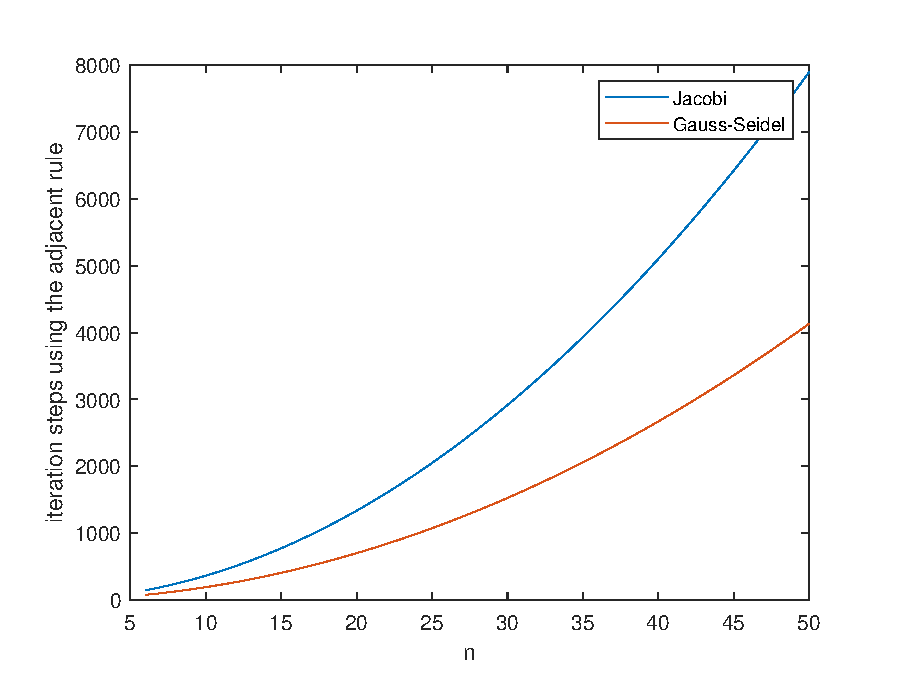
\includegraphics[width=14cm,height=10cm]{2.1_steps_adjacent_1.eps}
    \caption{The iteration steps using the adjacent rule and 1-norm}
\end{figure*}
\begin{figure*}[ht]
    \centering
    \includegraphics[width=14cm,height=10cm]{2.1_error_backward_1.eps}
    \caption{The numerical error using the backward rule and 1-norm}
\end{figure*}
\begin{figure*}[ht]
    \centering
    \includegraphics[width=14cm,height=10cm]{2.1_steps_backward_1.eps}
    \caption{The iteration steps using the backward rule and 1-norm}
\end{figure*}
\begin{figure*}[ht]
    \centering
    \includegraphics[width=14cm,height=10cm]{2.1_error_remaining_inf.eps}
    \caption{The numerical error using the remaining rule and inf-norm}
\end{figure*}
\begin{figure*}[ht]
    \centering
    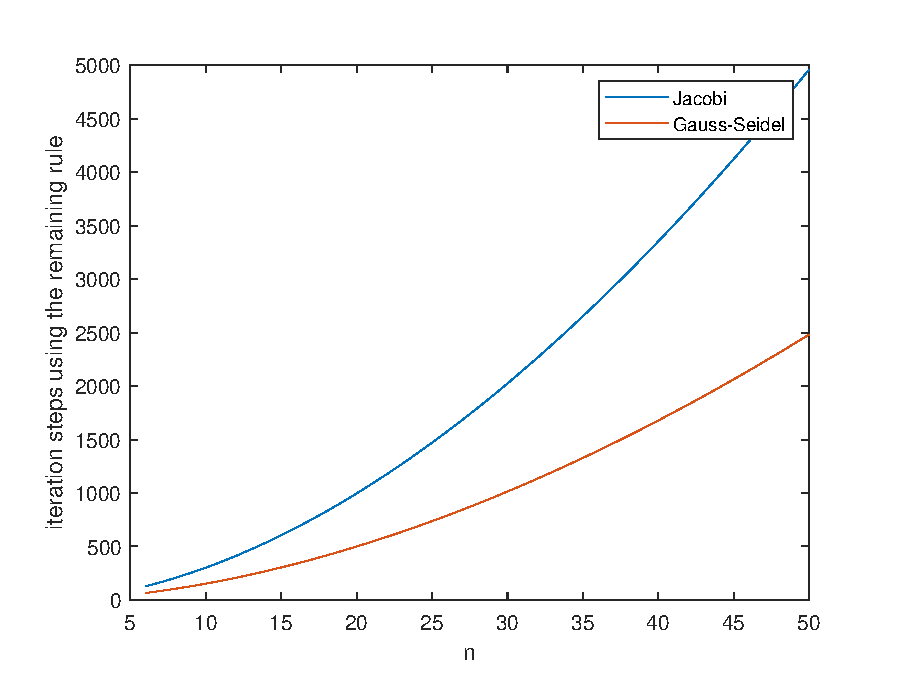
\includegraphics[width=14cm,height=10cm]{2.1_steps_remaining_inf.eps}
    \caption{The iteration steps using the remaining rule and inf-norm}
\end{figure*}
\begin{figure*}[ht]
    \centering
    \includegraphics[width=14cm,height=10cm]{2.1_error_adjacent_inf.eps}
    \caption{The numerical error using the adjacent rule and inf-norm}
\end{figure*}
\begin{figure*}[ht]
    \centering
    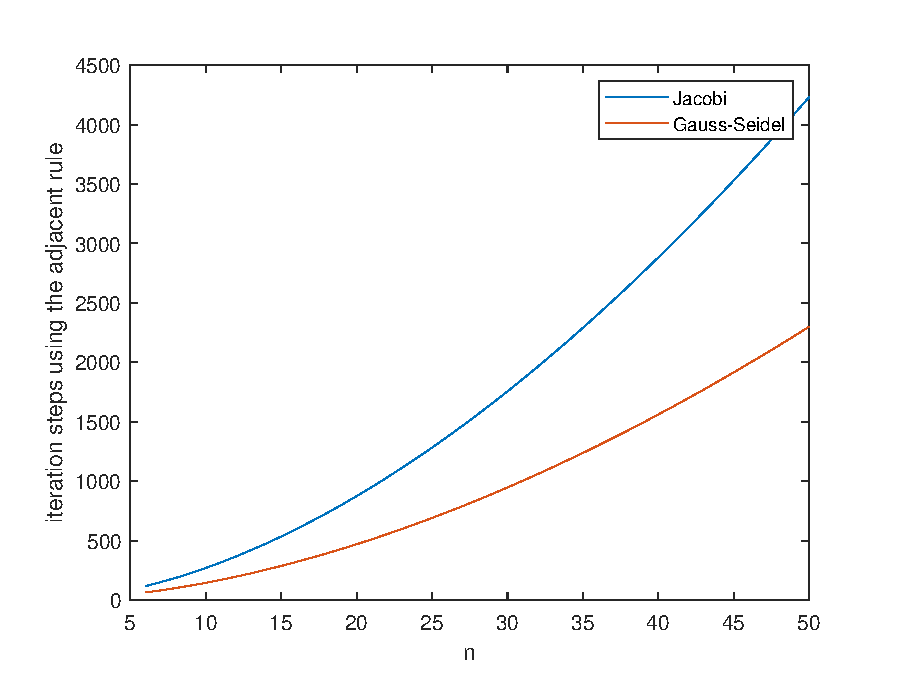
\includegraphics[width=14cm,height=10cm]{2.1_steps_adjacent_inf.eps}
    \caption{The iteration steps using the adjacent rule and inf-norm}
\end{figure*}
\begin{figure*}[ht]
    \centering
    \includegraphics[width=14cm,height=10cm]{2.1_error_backward_inf.eps}
    \caption{The numerical error using the backward rule and inf-norm}
\end{figure*}
\begin{figure*}[ht]
    \centering
    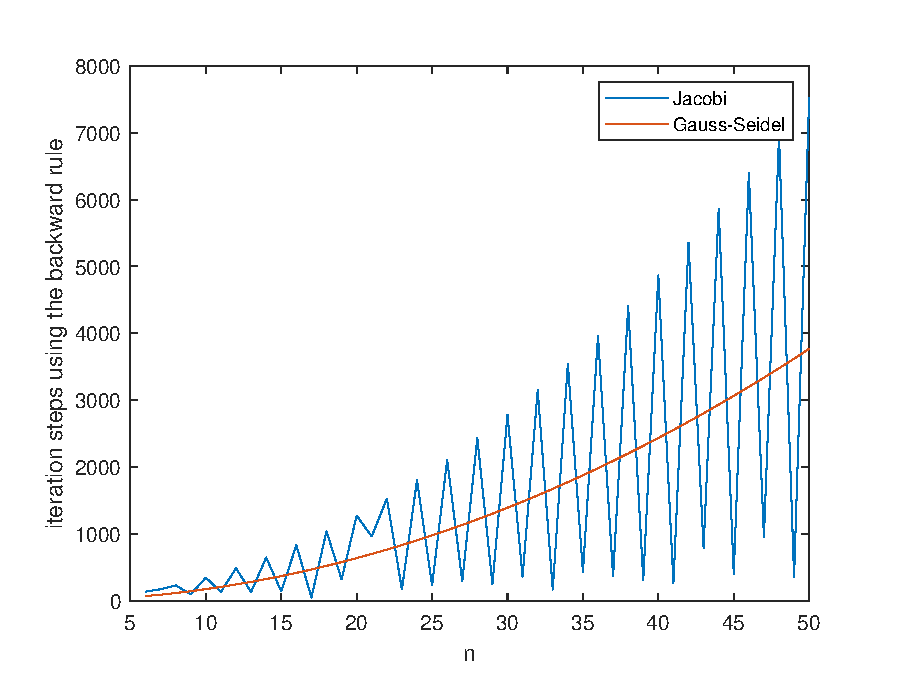
\includegraphics[width=14cm,height=10cm]{2.1_steps_backward_inf.eps}
    \caption{The iteration steps using the backward rule and inf-norm}
\end{figure*}

\begin{figure*}[ht]
    \centering
    \includegraphics[width=14cm,height=10cm]{2.3_error.eps}
    \caption{The numerical error of the 3 algorithms}
\end{figure*}
\begin{figure*}[ht]
    \centering
    \includegraphics[width=14cm,height=10cm]{2.3_remaining.eps}
    \caption{The remaining of the 3 algorithms}
\end{figure*}
\begin{figure*}[ht]
    \centering
    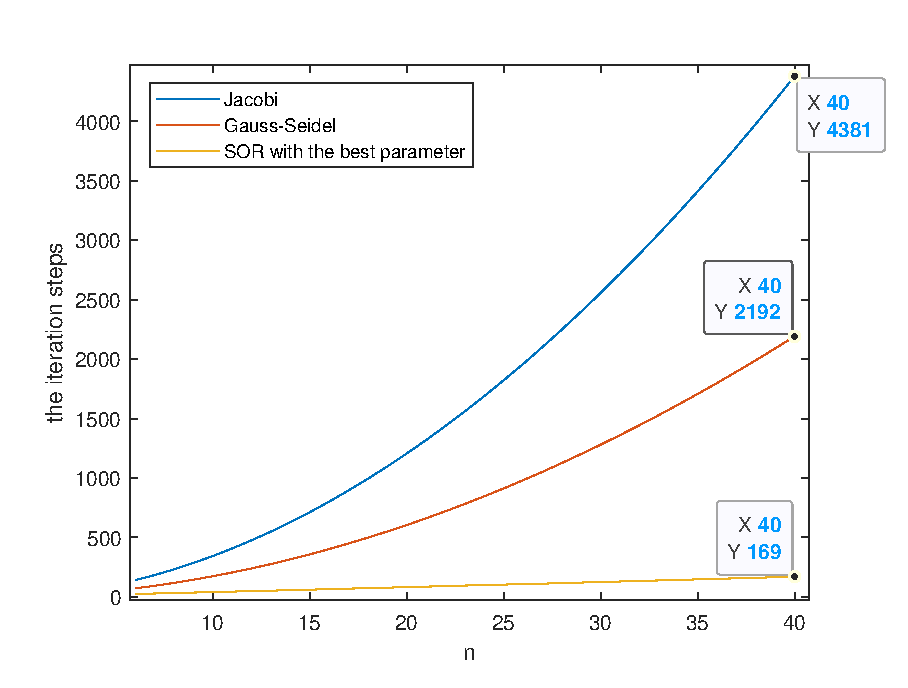
\includegraphics[width=14cm,height=10cm]{2.3_steps.eps}
    \caption{The iteration steps using the 3 algorithms}
\end{figure*}

\begin{figure*}[ht]
    \centering
    \includegraphics[width=14cm,height=10cm]{2.4_error.eps}
    \caption{The numerical error trend by changing m}
\end{figure*}
\begin{figure*}[ht]
    \centering
    \includegraphics[width=14cm,height=10cm]{2.4_remaining.eps}
    \caption{The remaining of different m}
\end{figure*}

\begin{figure*}[ht]
    \centering
    \includegraphics[width=14cm,height=10cm]{2.5_error.eps}
    \caption{The numerical trend of different m}
\end{figure*}
\begin{figure*}[ht]
    \centering
    \includegraphics[width=14cm,height=10cm]{2.5_remaining.eps}
    \caption{The remaining trend by changing m}
\end{figure*}

\begin{figure*}[ht]
    \centering
    \includegraphics[width=14cm,height=10cm]{2.6_error.eps}
    \caption{The numerical error in the case of n=50 and n=51 as iterating}
\end{figure*}
\begin{figure*}[ht]
    \centering
    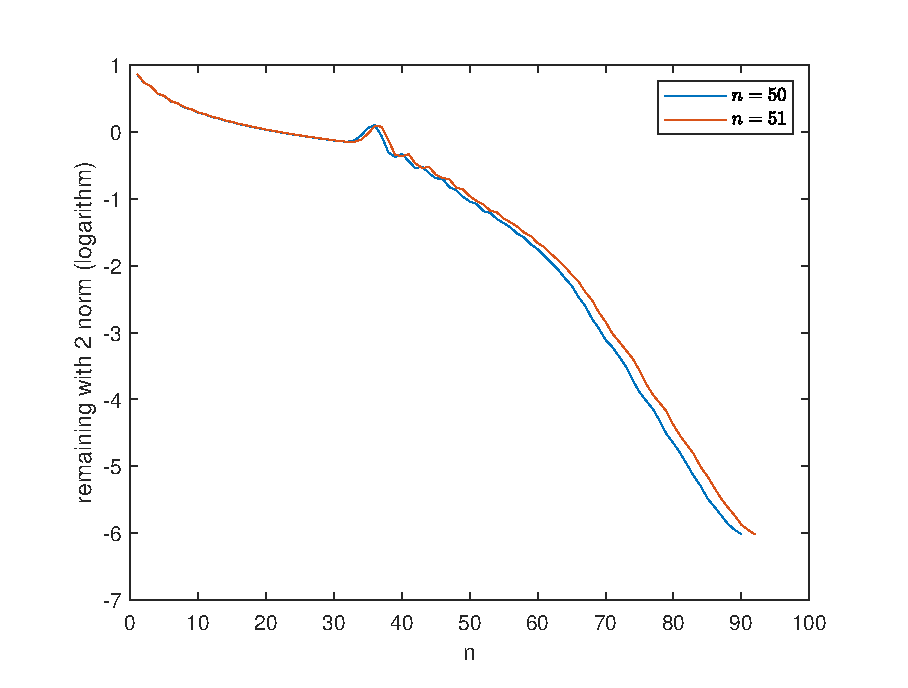
\includegraphics[width=14cm,height=10cm]{2.6_remaining.eps}
    \caption{The remaining in the case of n=50 and n=51 as iterating}
\end{figure*}
\begin{figure*}[ht]
    \centering
    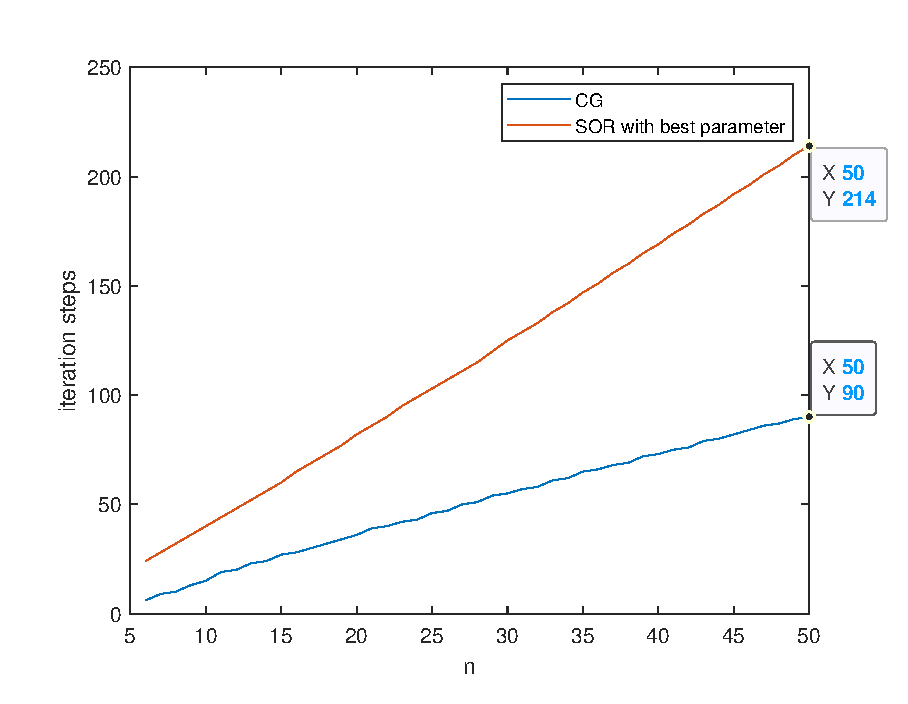
\includegraphics[width=14cm,height=10cm]{2.6_steps.eps}
    \caption{The iteration steps of CG method and SOR method with the best parameter}
\end{figure*}

    
\section*{参考文献}
[1]林成森. 数值计算方法(下册)[M]. 北京: 科学出版社, 2005.
\end{document}
